\newcommand{\base}{\ensuremath{\mathsf{base}}\xspace}
\newcommand{\lloop}{\ensuremath{\mathsf{loop}}\xspace}
\newcommand{\surf}{\ensuremath{\mathsf{surf}}\xspace}
\newcommand{\seg}{\ensuremath{\mathsf{seg}}\xspace}
\newcommand{\eqtopath}{\ensuremath{\mathsf{eqtopath}}\xspace}
\newcommand{\dpath}[4]{#3 =^{#1}_{#2} #4}
\newcommand{\susp}{\Sigma}
\newcommand{\north}{\mathsf{N}}
\newcommand{\south}{\mathsf{S}}
\newcommand{\merid}{\mathsf{merid}}
\newcommand{\Map}{\mathsf{Map}}

\chapter{Higher inductive types}
\label{cha:hits}

\section{Introduction to HITs}
\label{sec:intro-hits}

Like the general inductive types we discussed in Chapter~\ref{cha:induction}, \emph{higher inductive types} are a general schema for defining new types generated by some constructors.
But unlike ordinary inductive types, in defining a higher inductive type we may have ``constructors'' which generate not only \emph{points} of that type, but also \emph{paths} and higher paths in that type.
For instance, we can consider the higher inductive type $\Sn^1$ generated by
\begin{itemize}
\item A point $\base:\Sn^1$, and
\item A path $\lloop : {\id[\Sn^1]\base\base}$.
\end{itemize}
This should be regarded as entirely analogous to the definition of, for instance, $\bool$, as being generated by
\begin{itemize}
\item A point $0:\bool$ and
\item A point $1:\bool$,
\end{itemize}
or the definition of $\nat$ as generated by
\begin{itemize}
\item A point $0:\nat$ and
\item A function $s:\nat\to\nat$.
\end{itemize}
When we think of types as higher groupoids, the more general notion of ``generation'' is very natural:
since a higher groupoid is a ``multi-sorted object'' with paths and higher paths as well as points, we should allow ``generators'' in all dimensions.
However, there are some important points to be made regarding this generalization.

First of all, the word ``generation'' should be taken seriously, in the same sense that a group can be freely generated by some set.
In particular, because a higher groupoid comes with \emph{operations} on paths and higher paths, when such an object is ``generated'' by certain constructors, the operations will create more paths that don't come directly from the constructors themselves.
For instance, in the higher inductive type $\Sn^1$, the constructor $\lloop$ is not the only nontrivial path from $\base$ to $\base$; we have also $\lloop\ct\lloop$ and $\lloop\ct\lloop\ct\lloop$ and so on, as well as $\opp{\lloop}$, etc., all of which are different.
This may seem so obvious as to be not worth mentioning, but it is a departure from the behavior of ``ordinary'' inductive types, where one can expect to see nothing in the inductive type except what was ``put in'' directly by the constructors.

Secondly, this generation is really \emph{free} generation: higher inductive types do not technically allow us to impose ``axioms'', such as forcing $\lloop\ct\lloop$ to equal $\refl{\base}$.
However, in the world of $\infty$-groupoids, there is little difference between ``free generation'' and ``presentation'', since we can make two paths equal \emph{up to homotopy} by adding a new 2-dimensional generator relating them (e.g.\ a path $\lloop\ct\lloop = \refl{\base}$ in $\base=\base$).
We do then, of course, have to worry about whether this new generator should satisfy its own ``axioms'', and so on, but in principle any ``presentation'' can be transformed into a ``free'' one by making axioms into constructors.
As we will see, by adding ``truncation constructors'' we can use higher inductive types to express classical notions such as group presentations as well.

Thirdly, even though a higher inductive type contains ``constructors'' which generate \emph{paths in} that type, it is still an inductive definition of a \emph{single} type.
In particular, as we will see, it is the higher inductive type itself which will be given a universal property (expressed, as usual, by an induction principle), and \emph{not} its identity types.
The identity type of a higher inductive type retains the usual induction principle of any identity type (i.e.\ path induction), and does not acquire any new induction principle.

This implies that in general, it may be quite nontrivial to identify the identity types of a higher inductive type in any concrete way, in contrast to how in Chapter~\ref{cha:basics} we were able to give explicit descriptions of the behavior of identity types under all the traditional type forming operations.
For instance, are there any paths from $\base$ to $\base$ in $\Sn^1$ which are not simply composites of copies of $\lloop$ and its inverse?
Intuitively, it seems that the answer should be no (and it is), but proving this is not entirely trivial.
Indeed, such questions bring us rapidly to problems such as calculating the homotopy groups of spheres, a long-standing problem in algebraic topology for which no simple formula is known.
Homotopy type theory brings a new and powerful viewpoint to bear on such questions, but it also requires type theory to become as complex as the answers to these questions.

Fourthly, the ``dimension'' of the constructors (i.e.\ whether they output points, paths, paths between paths, etc.)\ does not have a direct connection to which dimensions the resulting type has nontrivial homotopy in.
As a simple example, if an inductive type $B$ has a constructor of type $A\to B$, then any paths and higher paths in $A$ will result in paths and higher paths in $B$, even though the constructor is not a ``higher'' constructor at all.
The same thing happens with higher constructors too: having a constructor of type $A\to (\id[B]xy)$ means not only that points of $A$ yield paths from $x$ to $y$ in $B$, but that paths in $A$ yield paths between these paths, and so on.
As we will see, this possibility is responsible for much of the power of higher inductive types.

On the other hand, it is even possible for constructors \emph{without} higher types in their inputs to generate ``unexpected'' higher paths.
For instance, in the 2-dimensional sphere $\Sn^2$ generated by
\begin{itemize}
\item A point $\base:\Sn^2$, and
\item A 2-dimensional path $\surf:\refl{\base} = \refl{\base}$ in ${\base=\base}$,
\end{itemize}
there is a nontrivial \emph{3-dimensional path} from $\refl{\refl{\base}}$ to itself.
Topologists will recognize this path as an incarnation of the \emph{Hopf fibration}.
From a category-theoretic point of view, this is the same sort of phenomenon as the fact mentioned above that $\Sn^1$ contains not only $\lloop$ but also $\lloop\ct\lloop$ and so on: it's just that in a \emph{higher} groupoid, there are \emph{operations} which raise dimension.
Indeed, we saw many of these operations back in \S\ref{sec:equality}: the associativity and unit laws are not just axioms but operations, whose inputs are 1-paths and whose outputs are 2-paths.


\section{Induction principles and dependent paths}
\label{sec:dependent-paths}

When we describe a higher inductive type such as the circle as being generated by certain constructors, we have to explain what this means by giving rules analogous to those for the basic type constructors from Chapter~\ref{cha:typetheory}.
The constructors themselves give the \emph{introduction} rules, but it requires a bit more thought to explain the \emph{elimination} rules.
In this book we will not attempt to give a general formulation of what constitutes a ``higher inductive definition'' and how to extract the elimination rule from such a definition --- indeed, this is a subtle question and the subject of current research.
Instead we will rely on some general informal discussion and numerous examples.

The non-dependent form of the eliminator is usually easy to describe: given any type equipped with the same structure with which the constructors equip the HIT in question, there is a function which maps the constructors to that structure.
For instance, in the case of $\Sn^1$, the non-dependent eliminator says that given any type $B$ equipped with a point $b:B$ and a path $\ell:b=b$, there is a function $f:\Sn^1\to B$ such that $f(\base)=b$ and $\ap f \lloop = \ell$ (the computation rules).

There is, however, a question of whether these computation rules are judgmental equalities or paths.
For ordinary inductive types, we had no qualms about making them judgmental; in that case one may argue that they are really \emph{definitional} equalities in the intuitive sense.
For higher inductive types, this is less clear, and it is likewise less clear to what extent these equalities can be made judgmental in the known set-theoretic models.
Moreover, since the operation $\apfunc f$ is not really a fundamental part of the type theory, but something that we \emph{defined} using the induction principle of identity types (and which we might have defined in some other, equivalent, way), it seems odd to refer to it explicitly in a judgmental equality.

There is generally consensus that the computational equalities for \emph{point} constructors, at least, should be judgmental.
In the example above, this means we have $f(\base)\jdeq b$.
This is unproblematic both philosophically and semantically.
Moreover, it greatly simplifies our lives, since otherwise the second computation rule $\ap f \lloop = \ell$ would not even be well-typed as a propositional equality; we would have to compose one side or the other with the specified identification of $f(\base)$ with $b$.
(Such problems do arise eventually, of course, when we come to talk about paths of higher dimension, but that will not be of great concern to us here.)
Thus, we will take the point-constructor computation rules to be judgmental, and those for paths and higher paths to be propositional.

Now, what about the dependent eliminator (the induction principle)?
Recall that for an ordinary inductive type $W$, to prove by induction that $\prd{x:W} P(x)$, we must specify for each constructor of $W$, an operation on $P$ which acts on the ``fibers'' above that constructor in $W$.
For instance, if $W$ is the natural numbers \nat, then to prove by induction that $\prd{x:\nat} P(x)$, we must specify
\begin{itemize}
\item An element $b:P(0)$ in the fiber over the constructor $0:\nat$, and
\item For each $n:\nat$, a function $P(n) \to P(s(n))$.
\end{itemize}
The second can be viewed as a function ``$P\to P$'' lying \emph{over} the constructor $s:\nat\to\nat$, generalizing how $b:P(0)$ lies over the constructor $0:\nat$.

By analogy, therefore, to prove that $\prd{x:\Sn^1} P(x)$, we should specify
\begin{itemize}
\item An element $b:P(\base)$ in the fiber over the constructor $\base:\nat$, and
\item A path from $b$ to $b$ ``lying over the constructor $\lloop:\base=\base$''.
\end{itemize}
The question is what it means to have a path ``lying over'' another path.
It definitely does \emph{not} mean simply a path $b=b$, since that would be a path in the fiber $P(\base)$ (topologically, a path lying over the \emph{constant} path at $\base$).

Actually, however, we have already answered this question in Chapter~\ref{cha:basics}: in the discussion preceeding \autoref{lem:mapdep} we concluded that a path from $u:P(x)$ to $v:P(y)$ lying over $p:x=y$ can be represented by a path $\trans p u = v$ in the fiber $P(y)$.
Since we will have a lot of use for such \emph{dependent paths} in this chapter, we introduce a special notation for them:
\[ (\dpath P p u v) \defeq (\transfib{P} p u = v). \]

\begin{rmk}
There are other possible ways to define dependent paths.
For instance, instead of $\trans p u = v$ we could consider $u = \trans{(\opp p)}{v}$.
We could also obtain it as a special case of a more general ``heterogeneous equality'', or with a direct definition as an inductive type family.
All these definitions result in equivalent types, so in that sense it doesn't very much matter much which we pick.
However, choosing $\trans p u = v$ as the definition makes it easiest to conclude other things about dependent paths, such as the fact that $\apdfunc{f}$ produces them, or that we can compute them in particular type families using the transport lemmas in \S\ref{sec:computational}.
\end{rmk}

With the notion of dependent paths in hand, we can now state more precisely the induction principle for $\Sn^1$: given $P:\Sn^1\to\type$ and
\begin{itemize}
\item An element $b:P(\base)$, and
\item A path $\ell : \dpath P \lloop b b$,
\end{itemize}
there is a function $f:\prd{x:\Sn^1} P(x)$ such that $f(\base)\jdeq b$ and $\apd f \lloop = \ell$.
In this situation, we may speak of defining $f$ by $f(\base)\defeq b$ and $\apd f \lloop \defeq \ell$, even though technically the latter is not a definitional equality.

Topologically, the induction principle for $\Sn^1$ can be visualized as shown in \autoref{fig:topS1ind}.
Given a fibration over the circle (which in the picture is a torus), to define a section of this fibration is the same as to give a point $b$ in the fiber over $\base$ along with a path from $b$ to $b$ lying over $\lloop$.
The way we interpret this type-theoretically, using our definition of dependent paths, is shown in \autoref{fig:ttS1ind}: the path from $b$ to $b$ over $\lloop$ is represented by a path from $\trans \lloop b$ to $b$ in the fiber over $\base$.

\begin{figure}
  \centering
  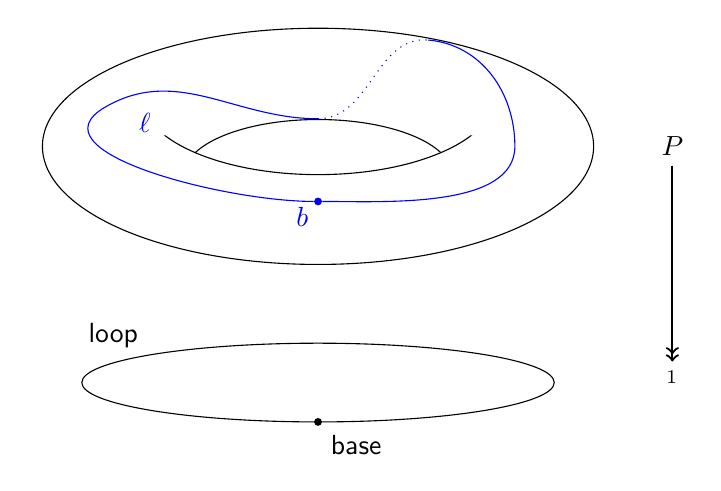
\begin{tikzpicture}
    \draw (0,0) ellipse (3 and .5);
    \draw (0,3) ellipse (3.5 and 1.5);
    \begin{scope}[yshift=4]
      \clip (-3,3) -- (-1.8,3) -- (-1.8,3.7) -- (1.8,3.7) -- (1.8,3) -- (3,3) -- (3,0) -- (-3,0) -- cycle;
      \draw[clip] (0,3.5) ellipse (2.25 and 1);
      \draw (0,2.5) ellipse (1.7 and .7);
    \end{scope}
    \node (P) at (4.5,3) {$P$};
    \node (S1) at (4.5,0) {$\Sn^1$};
    \draw[->>,thick] (P) -- (S1);
    \node[fill,circle,inner sep=1pt,label={below right:$\base$}] at (0,-.5) {};
    \node at (-2.6,.6) {$\lloop$};
    \node[fill,circle,blue,inner sep=1pt] (b) at (0,2.3) {};
    \node[blue] at (-.2,2.1) {$b$};
      \begin{scope}
        \draw[blue] (b) to[out=180,in=-150] (-2.7,3.5) to[out=30,in=180] (0,3.35);
        \draw[blue,dotted] (0,3.35) to[out=0,in=175] (1.4,4.35);
        \draw[blue] (1.4,4.35) to[out=-5,in=90] (2.5,3) to[out=-90,in=0,looseness=.8] (b);
      \end{scope}
      \node[blue] at (-2.2, 3.3) {$\ell$};
  \end{tikzpicture}
  \caption{The topological induction principle for $\Sn^1$}
  \label{fig:topS1ind}
\end{figure}

\begin{figure}
  \centering
  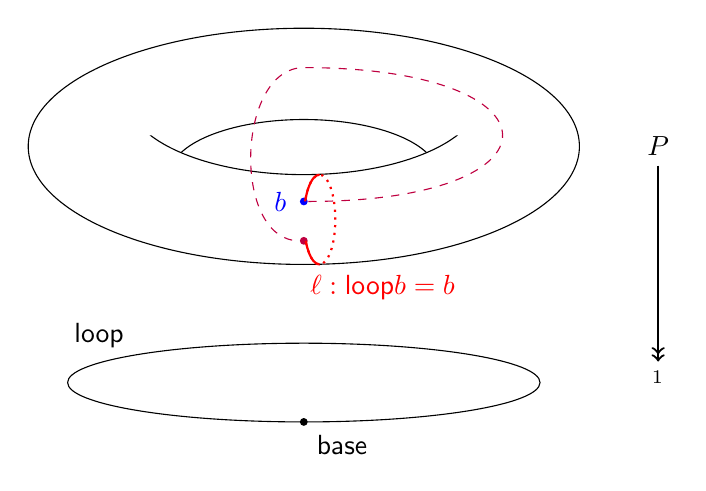
\begin{tikzpicture}
    \draw (0,0) ellipse (3 and .5);
    \draw (0,3) ellipse (3.5 and 1.5);
    \begin{scope}[yshift=4]
      \clip (-3,3) -- (-1.8,3) -- (-1.8,3.7) -- (1.8,3.7) -- (1.8,3) -- (3,3) -- (3,0) -- (-3,0) -- cycle;
      \draw[clip] (0,3.5) ellipse (2.25 and 1);
      \draw (0,2.5) ellipse (1.7 and .7);
    \end{scope}
    \node (P) at (4.5,3) {$P$};
    \node (S1) at (4.5,0) {$\Sn^1$};
    \draw[->>,thick] (P) -- (S1);
    \node[fill,circle,inner sep=1pt,label={below right:$\base$}] at (0,-.5) {};
    \node at (-2.6,.6) {$\lloop$};
    \node[fill,circle,blue,inner sep=1pt] (b) at (0,2.3) {};
      \node[blue] at (-.3,2.3) {$b$};
      \node[fill,circle,purple,inner sep=1pt] (tb) at (0,1.8) {};
      \draw[purple,dashed] (b) to[out=0,in=0,looseness=5] (0,4) to[out=180,in=180] (tb);
      \begin{scope}
        \clip (b) -- ++(.1,0) -- (.1,1.8) -- ++(-.2,0) -- ++(0,-1) -- ++(3,2) -- ++(-3,0) -- (-.1,2.3) -- cycle;
        \draw[red,dotted,thick] (.2,2.07) ellipse (.2 and .57);
        \begin{scope}
          % \draw[clip] (b) -- ++(.1,0) |- (tb) -- ++(-.2,0) -- ++(0,-1) -| ++(3,3) -| (b);
          \clip (.2,0) rectangle (-2,3);
          \draw[red,thick] (.2,2.07) ellipse (.2 and .57);
        \end{scope}
      \end{scope}
      \node[red] at (1,1.2) {$\ell: \trans \lloop b=b$};
  \end{tikzpicture}
  \caption{The type-theoretic induction principle for $\Sn^1$}
  \label{fig:ttS1ind}
\end{figure}

Of course, we expect to be able to prove the non-dependent elimination rule from the dependent one, by taking $P$ to be a constant type family.
This is in fact the case, although deriving the non-dependent computation rule for $\lloop$ (which refers to $\apfunc f$) from the dependent one (which refers to $\apdfunc f$) is surprisingly a little tricky.

\begin{lem}\label{thm:S1rec}
  If $A$ is a type together with $a:A$ and $p:\id[A]aa$, then there is a
  function $f:\Sn^1\to{}A$ with
  \begin{align*}
    f(\base)&\jdeq a \\
    \apfunc f(\lloop)&=p.
  \end{align*}
\end{lem}
\begin{proof}
  The type $(\dpath {x \mapsto A}{\lloop} a a)\jdeq (\transfib{x \mapsto A}{\lloop} a = a)$ is not the same as the type $\id[A]aa$.
  But it is equivalent to it, because by \autoref{thm:trans-trivial} we have $\transconst{A}{\lloop}{a} : \transfib{x \mapsto A}{\lloop} a= a$.
  Thus, given $a:A$ and $p:a=a$, we can consider the composite
  \[\transconst{A}{\lloop}{a} \ct p:(\dpath {x \mapsto A}\lloop aa).\]
  Applying the induction principle, we obtain $f:\Sn^1\to A$ such that
  \begin{alignat}{2}
    f(\base) &\jdeq a & \quad\text{and}\label{eq:S1recindbase}\\
    \apdfunc f(\lloop) &= \transconst{A}{\lloop}{a} \ct p.\label{eq:S1recindloop}
  \end{alignat}
  It remains to derive the equality $\apfunc f(\lloop)=p$.
  However, by \autoref{thm:apd-const}, we have
  \[\apdfunc f(\lloop) = \transconst{A}{\lloop}{f(\base)} \ct \apfunc f(\lloop).\]
  Combining this with~\eqref{eq:S1recindloop} and canceling the occurrences of $\transconstf$ (which are the same by~\eqref{eq:S1recindbase}), we obtain $\apfunc f(\lloop)=p$.
\end{proof}

Similarly, in this case we may speak of defining $f$ by $f(\base)\defeq a$ and $\ap f \lloop \defeq p$.
We also have an $\eta$-rule.

\begin{lem}
  If $A$ is a type and $f,g:\Sn^1\to{}A$ are two maps together with two
  equalities $p,q$:
  \begin{align*}
    p:f(\base)&=_Ag(\base)\\
    q:\map{f}\lloop&=^{\lambda{}x.\,x=_Ax}_p\map{g}\lloop
  \end{align*}
  Then for all $x:\Sn^1$ we have $f(x)=g(x)$.
\end{lem}
\begin{proof}
  This is just the induction principle for the type family $P(x)\defeq(f(x)=g(x))$.
\end{proof}

These two lemmas imply the expected universal property of the circle:

\begin{lem}\label{thm:S1ump}
  For any type $A$ we have a natural equivalence
  \[ (\Sn^1 \to A) \;\simeq\;
  \sm{x:A} (x=x).
  \]
\end{lem}
\begin{proof}
  We have a canonical function $f:(\Sn^1 \to A) \to \sm{x:A} (x=x)$ defined by $f(g) \defeq (g(\base),\ap g \lloop)$.
  The non-dependent eliminator shows that the fibers of $f$ are inhabited, while the $\eta$-rule shows that they are mere propositions.
  Hence they are contractible, so $f$ is an equivalence.
\end{proof}

Other higher inductive types also satisfy lemmas analogous to~\ref{thm:S1rec} and~\ref{thm:S1ump}; we will generally leave their proofs to the reader.
We now proceed to consider many examples.


\section{The interval}
\label{sec:interval}

The \emph{interval} $I$ is perhaps an even simpler higher inductive type than the circle.
It is generated by:
\begin{itemize}
\item a point $0:I$,
\item a point $1:I$, and
\item a path $\seg : \id[I]01$.
\end{itemize}
The recursion principle for the interval says that given a type $B$ along with
\begin{itemize}
\item a point $b_0:B$,
\item a point $b_1:B$, and
\item a path $s:b_0=b_1$,
\end{itemize}
there is a function $f:I\to B$ such that $f(0)\jdeq b_0$, $f(1)\jdeq b_1$, and $\ap f \seg = s$.
The induction principle says that given $P:I\to\type$ along with
\begin{itemize}
\item a point $b_0:P(0)$,
\item a point $b_1:P(1)$, and
\item a path $s:\dpath{P}{\seg}{b_0}{b_1}$,
\end{itemize}
there is a function $f:\prd{x:I} P(x)$ such that $f(0)\jdeq b_0$, $f(1)\jdeq b_1$, and $\apd f \seg = s$.

From the point of view of homotopy theory, of course, the interval is not really interesting:

\begin{lem}
  The type $I$ is contractible.
\end{lem}

\begin{proof}
  We will prove that for all $x:I$ we have $x=_I1$. In other words we want a
  function $f$ of type $\prd{x:I}(x=_I1)$. We begin to define $f$ in the following way:
  \begin{alignat*}{2}
    f(0)&\defeq \seg  &:0&=_I1\\
    f(1)&\defeq \refl1 &:1 &=_I1
  \end{alignat*}
  It remains to define $\apd{f}\seg$, which must have type $\seg =_\seg^{\lambda{}x.x=_I1}\refl 1$.
  By definition this type is $\trans\seg\seg=_{1=_I1}\refl1$, which in turn is equivalent to $\rev\seg\ct\seg=\refl1$.
  But there is a canonical term of that type, namely the proof that path inverses are in fact inverses.
\end{proof}

However, type-theoretically the interval is not completely boring, because it enables us to give an easy proof of function extensionality.

\begin{lem}
  If $f,g:A\to{}B$ are two functions such that $f(x)=g(x)$ for every $x:A$, then
  $f=g$ in the type $A\to{}B$.
\end{lem}

\begin{proof}
  Let's call the proof we have $p:\prd{x:A}(f(x)=g(x))$. For all $x:A$ we define
  a function $\widetilde{p}_x:I\to{}B$ by
  \begin{align*}
    \widetilde{p}_x(0) &= f(x) \\
    \widetilde{p}_x(1) &= g(x) \\
    \map{(\widetilde{p}_x)}\seg &= p(x)
  \end{align*}
  We now define $q:I\to(A\to{}B)$ by
  \[q(i)\defeq(\lambda{}x.\,\widetilde{p}_x(i))\]
  Then $q(0)$ is the function $\lambda{}x.\,\widetilde{p}_x(0)$, which is equal to $f$ because $\widetilde{p}_x(0)$ is defined by $f(x)$.
  Similarly, we have $q(1)=g$, and hence
  \[\map{q}\seg:f=_{(A\to{}B)}g \qedhere\]
\end{proof}


\section{Circles and spheres}
\label{sec:circle}

We have already discussed the circle $\Sn^1$ as the higher inductive type generated by
\begin{itemize}
\item A point $\base:\Sn^1$, and
\item A path $\lloop : {\id[\Sn^1]\base\base}$.
\end{itemize}
Its induction principle says that given $P:\Sn^1\to\type$ along with $b:P(\base)$ and $\ell :\dpath P \lloop b b$, we have $f:\prd{x:\Sn^1} P(x)$ with $f(\base)\jdeq b$ and $\apd f \lloop = \ell$.
Its non-dependent recursion principle says that given $B$ with $b:B$ and $\ell:b=b$, we have $f:\Sn^1\to B$ with $f(\base)\jdeq b$ and $\ap f \lloop = \ell$.

We observe that the circle is nontrivial.

\begin{lem}
  $\lloop\neq\refl{\base}$.
\end{lem}
\begin{proof}
  Suppose that $\lloop=\refl{\base}$.
  Then since for any type $A$ with $x:A$ and $p:x=x$, there is a function $f:\Sn^1\to A$ with $f(\base)\defeq x$ and $\ap f \lloop = p$, we have
  \[p = f(\lloop) = f(\refl{\base}) = \refl{x}.\]
  But this implies that every type is a set, which as we have seen is not the case (any universe containing \bool is not a set).
\end{proof}

The circle also has the following interesting property, which is useful as a source of counterexamples.

\begin{lem}\label{thm:S1-autohtpy}
  There exists an element of $\prd{x:\Sn^1} (x=x)$ which is not equal to $x\mapsto \refl{x}$.
\end{lem}
\begin{proof}
  We define $f:\prd{x:\Sn^1} (x=x)$ by $\Sn^1$-induction.
  When $x\jdeq \base$, we let $f(\base)\defeq \lloop$.
  Now when $x$ varies along $\lloop$, we must show that $\transfib{x\mapsto x=x}{\lloop}{\lloop} = \lloop$.
  However, in \S\ref{sec:compute-paths} we observed that $\transfib{x\mapsto x=x}{p}{q} = \opp{p} \ct q \ct p$, so what we have to show is that $\opp{\lloop} \ct \lloop \ct \lloop = \lloop$.
  But this is clear by canceling an inverse.

  To show that $f\neq (x\mapsto \refl{x})$, it suffices by function extensionality to show that $f(\base) \neq \refl{x}$.
  But $f(\base)=\lloop$, so this is just the previous lemma.
\end{proof}

For instance, this enables us to show that any universe which contains the circle cannot be a 1-type.
(Recall that we observed in \S\ref{sec:basics-sets} that any universe which contains \bool cannot be a set, i.e.\ a 0-type.)

\begin{cor}
  If the type $\Sn^1$ belongs to some universe \type, then \type is not a 1-type.
\end{cor}
\begin{proof}
  The type $\Sn^1=\Sn^1$ in \type is, by univalence, equivalent to the type $\eqv{\Sn^1}{\Sn^1}$ of autoequivalences of $\Sn^1$, so it suffices to show that $\eqv{\Sn^1}{\Sn^1}$ is not a set.
  Since being an equivalence is a mere proposition, it will suffice to show that the type ${\Sn^1}\to{\Sn^1}$ is not a set.
  For this, it will suffice to show that its equality type $\idfunc[\Sn^1] = \idfunc[\Sn^1]$ is not a mere proposition.
  But by function extensionality, this is equivalent to $\prd{x:\Sn^1} (x=x)$, which as we have seen in \autoref{thm:S1-autohtpy} contains two unequal elements.
\end{proof}

We have also mentioned that the 2-sphere $\Sn^2$ should be the higher inductive type generated by
\begin{itemize}
\item A point $\base:\Sn^2$, and
\item A 2-dimensional path $\surf:\refl{\base} = \refl{\base}$ in ${\base=\base}$.
\end{itemize}
The non-dependent recursion principle for $\Sn^2$ is not hard: it says that given $B$ with $b:B$ and $s:\refl b = \refl b$, we have $f:\Sn^2\to B$ with $f(\base)\jdeq b$ and $\aptwo f \surf = s$.
Here by ``$\aptwo f \surf$'' we must mean an extension of the functorial action of $f$ to two-dimensional paths, which can be stated precisely as follows.

\begin{lem}\label{thm:ap2}
  Given $f:A\to B$ and $x,y:A$ and $p,q:x=y$, and $r:p=q$, we have $\aptwo f r : \ap f p = \ap f q$.
\end{lem}
\begin{proof}
  By path induction, we may assume $p\jdeq q$ and $r$ is reflexivity.
  But then we may define $\aptwo f {\refl p} \defeq \refl{\ap f p}$.
\end{proof}

In order to state the general induction principle, we need a version of this lemma for dependent functions, which in turn requires a notion of dependent two-dimensional paths.
As before, there are many ways to define such a thing; one is by way of a two-dimensional version of transport.

\begin{lem}\label{thm:transport2}
  Given $P:A\to\type$ and $x,y:A$ and $p,q:x=y$ and $r:p=q$, for any $u:P(x)$ we have $\transtwo r u : \trans p u = \trans q u$.
\end{lem}
\begin{proof}
  By path induction.
\end{proof}

Now suppose given $x,y:A$ and $p,q:x=y$ and $r:p=q$ and also points $u:P(x)$ and $v:P(y)$ and dependent paths $h:\dpath P p u v$ and $k:\dpath P q u v$.
By our definition of dependent paths, this means $h:\trans p u = v$ and $k:\trans q u = v$.
Thus, it is reasonable to define the type of dependent 2-paths over $r$ to be
\[ (\dpath P r h k )\defeq (h = \transtwo r u \ct k). \]
We can now state the dependent version of \autoref{thm:ap2}.

\begin{lem}\label{thm:apd2}
  Given $P:A\to\type$ and $x,y:A$ and $p,q:x=y$ and $r:p=q$ and a function $f:\prd{x:A} P(x)$, we have
  $\apdtwo f r : \dpath P r {\apd f p}{\apd f q}$.
\end{lem}
\begin{proof}
  Path induction.
\end{proof}

Now we can state the induction principle for $\Sn^2$: given $P:\Sn^2\to P$ with $b:P(\base)$ and $s:\dpath P \surf {\refl b}{\refl b}$, there is a function $f:\prd{x:\Sn^2} P(x)$ such that $f(\base)\jdeq b$ and $\apdtwo f \surf = s$.

Of course, this explicit approach will get more and more complicated as we go up in dimension.
Thus, if we want to define $n$-spheres for all $n$, we need some more systematic idea.
One approach is to work with $n$-fold loops directly, rather than $n$-fold paths.

We write $\type_* \defeq \sm{A:\type} A$ for the type of \emph{pointed types} (in the universe \type); its elements are pairs $(A,a)$ where $A:\type$ and $a:A$.
Now we have a function $\Omega : \type_* \to \type_*$ called the \textbf{loop space}, defined by
\[ \Omega(A,a) \defeq \big((\id[A]aa),\refl a\big). \]
We define the $n$-fold loop space $\Omega^n : \type_* \to \type_*$ by iteration:
\begin{align*}
\Omega^0(A,a) &\defeq (A,a)\\
\Omega^{n+1}(A,a) &\defeq \Omega(\Omega^n(A,a))
\end{align*}
Now we can define the $n$-sphere $\Sn^n$ to be the higher inductive type generated by
\begin{itemize}
\item A point $\base:\Sn^n$, and
\item An $n$-fold loop $\lloop_n : \Omega^n(\Sn^n,\base)$.
\end{itemize}
In order to write down the induction principle for this presentation, we would need to define a notion of ``dependent $n$-loop'', along with the action of dependent functions on $n$-loops.
We leave this to the reader (see \autoref{ex:nspheres}); in the next section we will discuss a different way to define the spheres that is sometimes more tractable.


\section{Suspensions}
\label{sec:suspension}

The \textbf{suspension} of a type $A$ is the universal way of making the points of $A$ into paths (and hence the paths in $A$ into 2-paths, and so on).
It is a type $\susp A$ defined by the following generators:
\begin{itemize}
\item a point $\north:\susp A$,
\item a point $\south:\susp A$, and
\item a function $\merid:A \to (\id[\susp A]\north\south)$.
\end{itemize}
The names are intended to suggest a ``globe'' of sorts, with a north pole, a south pole, and an $A$'s worth of meridians from one to the other.
Indeed, as we will see, if $A=\Sn^1$, then its suspension is equivalent to the surface of an ordinary sphere, $\Sn^2$.

The recursion principle for $\susp A$ says that given a type $B$ together with points $n,s:B$ and a function $m:A \to (n=s)$, we have a function $f:\susp A \to B$ such that $f(\north)\jdeq n$ and $f(\south)\jdeq s$, and for all $a:A$ we have $\ap f {\merid(a)} = m(a)$.
The induction principle says that given $P:\susp A \to \type$ together with
\begin{itemize}
\item a point $n:P(\north)$,
\item a point $s:P(\south)$, and
\item for each $a:A$, a path $m(a):\dpath P{\merid(a)}ns$,
\end{itemize}
there exists a function $f:\prd{x:\susp A} P(x)$ such that $f(\north)\jdeq n$ and $f(\south)\jdeq s$ and for each $a:A$ we have $\apd f {\merid(a)} = m(a)$.

Our first observation about suspension is that it gives another way to define the circle.

\begin{lem}\label{thm:suspbool}
  $\eqv{\susp\bool}{\Sn^1}$.
\end{lem}
\begin{proof}
  Define $f:\susp\bool\to\Sn^1$ by recursion such that $f(\north)\defeq \base$ and $f(\south)\defeq\base$, while $\ap f{\merid(0)}=\lloop$ but $\ap f{\merid(1)} = \refl{\base}$.
  Define $g:\Sn^1\to\susp\bool$ by recursion such that $g(\base)\defeq \north$ and $\ap g \lloop = \merid(0) \ct \opp{\merid(1)}$.
  We now show that $f$ and $g$ are quasi-inverses.

  First we show by induction that $g(f(x))=x$ for all $x:\susp \bool$.
  If $x\jdeq\north$, then $g(f(\north)) \jdeq g(\base)\jdeq \north$, so we have $\refl{\north} : g(f(\north))=\north$.
  If $x\jdeq\south$, then $g(f(\south)) \jdeq g(\base)\jdeq \north$, and we choose the equality $\merid(1) : g(f(\south)) = \south$.
  It remains to show that for any $y:\bool$, these equalities are preserved as $x$ varies along $\merid(y)$, which is to say that when $\refl{\north}$ is transported along $\merid(y)$ it yields $\merid(1)$.
  By transport in path spaces and pulled back fibrations, this means we are to show that
  \[ \opp{\ap g {\ap f {\merid(y)}}} \ct \refl{\north} \ct \merid(y) = \merid(1). \]
  Of course, we may cancel $\refl{\north}$.
  Now by \bool-induction, we may assume either $y\jdeq 0$ or $y\jdeq 1$.
  If $y\jdeq 0$, then we have
  \begin{align*}
    \opp{\ap g {\ap f {\merid(0)}}} \ct \merid(0)
    &= \opp{\ap g {\lloop}} \ct \merid(0)\\
    &= \opp{\merid(0) \ct \opp{\merid(1)}} \ct \merid(0)\\
    &= \merid(1) \ct \opp{\merid(0)} \ct \merid(0)\\
    &= \merid(1)
  \end{align*}
  while if $y\jdeq 1$, then we have
  \begin{align*}
    \opp{\ap g {\ap f {\merid(1)}}} \ct \merid(1)
    &= \opp{\ap g {\refl{\base}}} \ct \merid(1)\\
    &= \opp{\refl{\north}} \ct \merid(1)\\
    &= \merid(1).
  \end{align*}
  Thus, for all $x:\susp \bool$, we have $g(f(x))=x$.

  Now we show by induction that $f(g(x))=x$ for all $x:\Sn^1$.
  If $x\jdeq \base$, then $f(g(\base))\jdeq f(\north)\jdeq\base$, so we have $\refl{\base} : f(g(\base))=\base$.
  It remains to show that this equality is preserved as $x$ varies along $\lloop$, which is to say that it is transported along $\lloop$ to itself.
  Again, by transport in path spaces and pulled back fibrations, this means to show that
  \[ \opp{\ap f {\ap g {\lloop}}} \ct \refl{\base} \ct \lloop = \refl{\base}.\]
  However, we have
  \begin{align*}
    \ap f {\ap g {\lloop}} &= \ap f {\merid(0) \ct \opp{\merid(1)}}\\
    &= \ap f {\merid(0)} \ct \opp{\ap f {\merid(1)}}\\
    &= \lloop \ct \refl{\base}
  \end{align*}
  so this follows easily.
\end{proof}

Topologically, the two-point space \bool is also known as the \emph{0-dimensional sphere}, $\Sn^0$.
(For instance, it is the space of points at distance $1$ from the origin in $\mathbb{R}^1$, just as the topological 1-sphere is the space of points at distance $1$ from the origin in $\mathbb{R}^2$.)
Thus, \autoref{thm:suspbool} can be phrased suggestively as $\eqv{\susp\Sn^0}{\Sn^1}$.
In fact, this pattern continues: we can define all the spheres inductively by
\begin{equation}\label{eq:Snsusp}
\begin{split}
  \Sn^0 &\defeq \bool\\
  \Sn^{n+1} &\defeq \susp \Sn^n.
\end{split}
\end{equation}
To prove that this is correct would require making explicit the definition of $\Sn^n$ from the previous section, but we can motivate it as follows.
If $(A,a_0)$ and $(B,b_0)$ are pointed types (with basepoints often left implicit), let $\Map_*(A,B)$ denote the type of based maps:
\[ \Map_*(A,B) \defeq \sm{f:A\to B} (f(a_0)=b_0). \]
Note that any type $A$ gives rise to a pointed type $A_+ \defeq A+\unit$ with basepoint $\inr(\ttt)$; this is called \emph{adjoining a disjoint basepoint}.

\begin{lem}
  For a type $A$ and a pointed type $(B,b_0)$, we have
  \[ \eqv{\Map_*(A_+,B)}{(A\to B)} \]
\end{lem}
Note that on the right we have the ordinary type of \emph{unbased} functions from $A$ to $B$.
\begin{proof}
  From left to right, given $f:A_+ \to B$ with $p:f(\inr(\ttt)) = b_0$, we have $f\circ \inl : A \to B$.
  And from right to left, given $g:A\to B$ we define $g':A_+ \to B$ by $g'(\inl(a))\defeq g(a)$ and $g'(\inr(u)) \defeq b_0$.
  We leave it to the reader to show that these are quasi-inverse operations.
\end{proof}

In particular, note that $\eqv{\bool}{\unit_+}$.
Thus, for any pointed type $B$ we have
\[{\Map_*(\bool,B)} \simeq {(\unit \to B)}\simeq B.\]

Now recall that the loop space operation $\Omega$ acts on pointed types, with definition $\Omega(A,a_0) \defeq (\id[A]{a_0}{a_0},\refl{a_0})$.
We can also make the suspension $\susp$ act on pointed types, by $\susp(A,a_0)\defeq (\susp A,\north)$.

\begin{lem}
  For pointed types $(A,a_0)$ and $(B,b_0)$ we have
  \[ \eqv{\Map_*(\susp A, B)}{\Map_*(A,\Omega B)}.\]
\end{lem}
\begin{proof}
  From left to right, given $f:\susp A \to B$ with $p:f(\north) = b_0$, we define $g:A \to \Omega B$ by
  \[g(a) \defeq \opp p \ct \ap f{\merid(a) \ct \opp{\merid(a_0)}} \ct p.\]
  Then we have
  \begin{align*}
    g(a_0) &\jdeq \opp p \ct \ap f{\merid(a_0) \ct \opp{\merid(a_0)}} \ct p\\
    &= \opp p \ct \ap f{\refl{\north}} \ct p\\
    &= \opp p \ct p\\
    &= \refl{b_0}.
  \end{align*}
  Thus, denoting this path by $q:g(a_0)=\refl{b_0}$, we have $(g,q):\Map_*(A,\Omega B)$.

  On the other hand, from right to left, given $g:A\to \Omega B$ and $q:g(a_0)=\refl{b_0}$, we define $f:\susp A \to B$ by $\susp$-recursion, such that $f(\north)\defeq b_0$ and $f(\south)\defeq b_0$ and
  \[ \ap f {\merid(a)} = g(a). \]
  Then we can simply take $p$ to be $\refl{b_0} : f(\north)= b_0$.

  Now given $(f,p)$, by passing back and forth we obtain $(f',p')$ where $f'$ is defined by $f'(\north)\jdeq b_0$ and $f'(\south)\jdeq b_0$ and
  \[ \ap {f'} {\merid(a)} = \opp p \ct \ap f{\merid(a) \ct \opp{\merid(a_0)}} \ct p, \]
  while $p' \jdeq \refl{b_0}$.
  To show $f=f'$, by function extensionality it suffices to show $f(x)=f'(x)$ for all $x:\susp A$, so we can use $\susp$-induction.
  First, we have
  \begin{equation}
    f(\north) \overset{p}{=} b_0 \jdeq f'(\north)\label{eq:ffprime-north}
  \end{equation}
  Second, we have
  \[f(\south) \overset{\opp{\ap f {\merid(a_0)}}}{=} f(\north) \overset{p}{=} b_0 \jdeq f'(\south).\]
  And thirdly, as $x$ varies along $\merid(a)$ we must show that the following diagram commutes (invoking the definition of $\ap{f'}{\merid(a)}$):
  \[ \xymatrix{
    f(\north) \ar[rrr]^{p} \ar[ddd]_{f(\merid(a))} &&&
    b_0 \ar@{=}[r] &
    f'(\north) \ar[d]^{\opp p}\\
    &&&& f(\north) \ar[d]^{\ap f{\merid(a) \ct \opp{\merid(a_0)}}}\\
    &&&& f(\north) \ar[d]^p\\
    f(\south) \ar[rr]_{\opp{\ap f {\merid(a_0)}}} &&
    f(\north) \ar[r]_p &
    b_0 \ar@{=}[r] &
    f'(\south) }
  \]
  This is clear.
  Thus, to show that $(f,p)=(f',p')$, it remains only to show that $p$ is identified with $p'$ when transported along this equality $f=f'$.
  Since the type of $p$ is $f(\north)=b_0$, this means essentially that when $p$ is composed on the left with the inverse of the equality~\eqref{eq:ffprime-north}, it becomes $p'$.
  But this is obvious, since~\eqref{eq:ffprime-north} is just $p$ itself, while $p'$ is reflexivity.

  On the other side, suppose given $(g,q)$.
  By passing back and forth we obtain $(g',q')$ with
  \begin{align*}
    g'(a) &= \opp{\refl{b_0}} \ct g(a) \ct \opp{g(a_0)} \ct \refl{b_0}\\
    &= g(a) \ct \opp{g(a_0)}\\
    &= g(a)
  \end{align*}
  using $q:g(a_0) = \refl{b_0}$ in the last equality.
  Thus, $g'=g$ by function extensionality, so it remains to show that when transported along this equality $q$ is identified with $q'$.
  At $a_0$, the induced equality $g(a_0)=g'(a_0)$ consists essentially of $q$ itself, while the definition of $q'$ involves only canceling inverses and reflexivities.
  Thus, some tedious manipulations of naturality finish the proof.
\end{proof}

In particular, for the spheres defined as in~\eqref{eq:Snsusp} we have
\[ \Map_*(\Sn^n,B) \simeq \Map_*(\Sn^{n-1}, \Omega B) \simeq \cdots \simeq \Map_*(\bool,\Omega^n B) \simeq \Omega^n B. \]
Thus, these spheres $\Sn^n$ have the universal property that we would expect from the spheres defined directly in terms of $n$-fold loops as in \S\ref{sec:circle}.


\section{Cell complexes}
\label{sec:cell-complexes}

In classical topology, a \textbf{cell complex} is a space obtained by successively attaching discs along their boundaries.
It is called a \textbf{CW complex} if the boundary of an $n$-dimensional disc is constrained to lie in the discs of dimension strictly less than $n$ (the $(n-1)$-skeleton).

Any finite CW complex can be presented as a higher inductive type, by turning $n$-dimensional discs into $n$-dimensional paths and partitioning the image of the attaching map into a ``source'' and a ``target'', with each written as a composite of lower-dimensional paths.
Our explicit definitions of $\Sn^1$ and $\Sn^2$ in \S\ref{sec:circle} had this form.

Another example is the torus $T^2$, which is generated by:
\begin{itemize}
\item a point $b:T^2$,
\item a path $p:b=b$,
\item another path $q:b=b$, and
\item a 2-path $t: p\ct q = q \ct p$.
\end{itemize}
Perhaps the easiest way to see that this is a torus is to start with a rectangle, having four corners $a,b,c,d$, four edges $p,q,r,s$, and an interior which is manifestly a 2-path $t$ from $p\ct q$ to $r\ct s$:
\begin{equation*}
  \vcenter{\xymatrix{
      a\ar[r]^p\ar[d]_r \ar@{}[dr]|{\Downarrow t} &
      b\ar[d]^q\\
      c\ar[r]_s &
      d
      }}
\end{equation*}
Now identify the edge $r$ with $q$ and the edge $s$ with $p$, resulting in also identifying all four corners.
Topologically, this identification can be seen to produce a torus.

The induction principle for the torus is the trickiest of any we've written out so far.
Given $P:T^1\to\type$, we require
\begin{itemize}
\item A point $b':P(b)$,
\item A path $p' : \dpath P p b b$,
\item A path $q' : \dpath P q b b$, and
\item A 2-path $t'$ between the ``composites'' $p'\ct q'$ and $q'\ct p'$, lying over $t$.
\end{itemize}
In order to make sense of this last datum, we need a composition operation for dependent paths, but this is not hard to define.
Then the induction principle gives a function $f:\prd{x:T^2} P(x)$ such that $f(b)\jdeq b'$ and $\apd f {p} = p'$ and $\apd f {q} = q'$ and something like ``$\apd f t = t'$''.
However, this is not well-typed as it stands, firstly because the equalities $\apd f {p} = p'$ and $\apd f {q} = q'$ are not judgmental, and secondly because $\apdfunc f$ only preserves path concatenation up to homotopy.
We leave the details to the reader (see \autoref{ex:torus}).

Of course, another definition of the torus is $T^2 \defeq \Sn^1 \times \Sn^1$.
The cell-complex definition, however, generalizes easily to other spaces without such descriptions, such as the Klein bottle, the projective plane, etc.


\section{Pushouts}
\label{sec:colimits}

From a category-theoretic point of view, one of the important aspects of any foundational system is the ability to construct limits and colimits.
In set-theoretic foundations, these are limits and colimits of sets, whereas in our case they will be limits and colimits of \emph{types}.
We have seen in \S\ref{sec:universal-properties} that cartesian product types have the correct universal property of a categorical product of types, and in \autoref{ex:coprod-ump} that coproduct types likewise have their expected universal property.

More general limits can be constructed using identity types and $\Sigma$-types, e.g.\ the pullback of $f:A\to C$ and $g:B\to C$ can be defined by $\sm{a:A}{b:B} (f(a)=g(b))$.
However, more general \emph{colimits} require identifying elements coming from different types, for which higher inductives are well-adapted.
Since all our constructions are homotopy-invariant, our colimits will all be \emph{homotopy colimits}, but we drop the ubiquitous adjective in the interests of conciseness.

In this section we discuss \emph{pushouts}, as perhaps the simplest and one of the most useful colimits.
Indeed, one expects all finite colimits to be constructible from pushouts and finite coproducts.
It is also possible to give a direct construction of more general colimits using higher inductive types, but this is somewhat technical, and also not completely satisfactory since we do not yet have a good fully general notion of homotopy coherent diagrams.

Suppose given a span of types and functions:
\[\Ddiag=\;\vcenter{\xymatrix{C \ar^g[r] \ar_f[d] & B \\ A & }}\]
The \textbf{pushout} of this span is the higher inductive type $A\sqcup^CB$ presented by
\begin{itemize}
\item a function $\inl:A\to A\sqcup^CB$,
\item a function $\inr:B \to A\sqcup^CB$, and
\item for each $c:C$ a path $\glue(c):(\inl(f(c))=\inr(g(c)))$.
\end{itemize}
In other words, $A\sqcup^CB$ is the disjoint union of $A$ and $B$, together with for every $c:C$ a witness that $f(c)$ and $g(c)$ are equal.
The recursion principle says that if $D$ is another type, we can define a map $s:A\sqcup^CB\to{}D$ by defining
\begin{itemize}
\item for each $a:A$, the value of $s(\inl(a)):D$,
\item for each $b:B$, the value of $s(\inr(b)):D$, and
\item for each $c:C$, the value of $\mapfunc{s}(\glue(c)):s(\inl(f(c)))=s(\inr(g(c)))$.
\end{itemize}
We leave it to the reader to formulate the induction principle.
It also implies the $\eta$-rule that if $s,s':A\sqcup^CB\to{}D$ are two maps such that
\begin{align*}
  s(\inl(a))&=s'(\inl(a))\\
  s(\inr(b))&=s'(\inr(b))\\
  \mapfunc{s}(\glue(c))&=\mapfunc{s'}(\glue(c))
  \qquad\text{(modulo the previous two equalities)}
\end{align*}
for every $a,b,c$, then $s=s'$.

\begin{rmk}
  Note that if $A\jdeq B\jdeq\unit$, then the above pushout is essentially the same as the suspension of the type $C$.
  This will be useful in Chapter~\ref{cha:homotopy}.
\end{rmk}

To formulate the universal property of a pushout, we introduce the following.

\begin{defn}
  Given functions $A \xleftarrow{f} C \xrightarrow{g} B$ and a type $D$, a \textbf{cocone under $\Ddiag$ with base $D$} consists of functions $i:A\to{}D$ and $j:B\to{}D$ and a homotopy $h : \prd{c:C} (i(f(c))=j(g(c)))$:
  \[\uppercurveobject{{ }}\lowercurveobject{{ }}\twocellhead{{ }}
  \xymatrix{C \ar^g[r] \ar_f[d] \drtwocell{^h} & B \ar^j[d] \\ A \ar_i[r] & D
  }\]
  We denote by $\cocone{\Ddiag}{D}$ the type of all such cocones, i.e.
  \[ \cocone{\Ddiag}{D} \defeq
  \sm{i:A\to D}{j:B\to D} \prd{c:C} (i(f(c))=j(g(c))).
  \]
\end{defn}

Of course, there is a canonical cocone under $\Ddiag$ with base $A\sqcup^C B$ consisting of $\inl$, $\inr$, and $\glue$.
\[\uppercurveobject{{ }}\lowercurveobject{{ }}\twocellhead{{ }}
\xymatrix{C \ar^g[r] \ar_f[d] \drtwocell{^\glue\ \ } & B \ar^\inr[d] \\
  A \ar_-\inl[r] & A\sqcup^CB }\]
The following lemma says that this is the universal such cocone.

\begin{lem}\label{thm:pushout-ump}
  For any type $E$, there is an equivalence
  \[ (A\sqcup^C B \to E) \;\simeq\; \cocone{\Ddiag}{E}. \]
\end{lem}
\begin{proof}
  Let's consider an arbitrary type $E:\type$.
  There is a canonical function
  \[\function{(A\sqcup^CB\to{}E)}{\cocone{\Ddiag}{E}}
  {t}{\composecocone{t}c_\sqcup}\]
  defined by sending $(i,j,h)$ to $(t\circ{}i,t\circ{}j,\mapfunc{t}\circ{}h)$.
  We will show that this is an equivalence.

  Firstly, given a $c=(i,j,h):\cocone{\mathscr{D}}{E}$, we need to construct a
  map $\mathsf{s}(c)$ from $A\sqcup^CB$ to $E$.
  \[\uppercurveobject{{ }}\lowercurveobject{{ }}\twocellhead{{ }}
  \xymatrix{C \ar^g[r] \ar_f[d] \drtwocell{^h} & B \ar^{j}[d] \\
    A \ar_-{i}[r] & E }\]
 The map $\mathsf{s}(c)$ is defined in the following way
  \begin{align*}
    \mathsf{s}(c)(\inl(a))&=i(a)\\
    \mathsf{s}(c)(\inr(b))&=j(b)\\
    \mapfunc{\mathsf{s}(c)}(\glue(x))&=h(x)\\
  \end{align*}
We have defined a map
\[\function{\cocone{\Ddiag}{E}}{(A\sqcup^BC\to{}E)}{c}{\mathsf{s}(c)}\]
and we need to prove that this map is an inverse to
$t\mapsto{}\composecocone{t}c_\sqcup$.
On the one hand, if $c=(i,j,h):\cocone{\Ddiag}{E}$, we have
\begin{align*}
  \composecocone{\mathsf{s}(c)}c_\sqcup & =
  (\mathsf{s}(c)\circ\inl,\mathsf{s}(c)\circ\inr,
  \mapfunc{\mathsf{s}(c)}\circ\glue) \\
  & = (\lambda{}a^A.\mathsf{s}(c)(\inl(a)),\lambda{}b^B.\mathsf{s}(c)(\inr(b)),
  \lambda{}x^C.\mapfunc{\mathsf{s}(c)}(\glue(x))) \\
  & = (\lambda{}a^A.i(a),\lambda{}b^B.j(b),
  \lambda{}x^C.h(x)) \\
  & = (i, j, h) \\
  & = c
\end{align*}

On the other hand, if $t:A\sqcup^BC\to{}E$, we want to prove that
$\mathsf{s}(\composecocone{t}c_\sqcup)=t$.
For $a:A$, we have
\[\mathsf{s}(\composecocone{t}c_\sqcup)(\inl(a))=t(\inl(a))\]
because the first component of $\composecocone{t}c_\sqcup$ is $t\circ\inl$. In
the same way, for $b:B$ we have
\[\mathsf{s}(\composecocone{t}c_\sqcup)(\inr(b))=t(\inr(b))\]
and for $x:C$ we have
\[\mapfunc{\mathsf{s}(\composecocone{t}c_\sqcup)}(\glue(x))
=\mapfunc{t}(\glue(x))\]
hence $\mathsf{s}(\composecocone{t}c_\sqcup)=t$.

This proves that $c\mapsto\mathsf{s}(c)$ is a quasi-inverse to $t\mapsto{}\composecocone{t}c_\sqcup$, as desired.
\end{proof}

We will discuss pushouts further in Chapter~\ref{cha:homotopy}.


\section{Truncations}
\label{sec:truncations}


\section{Quotients}
\label{sec:quotients}

Both as HIT and impredicatively.

\section{Free algebras}
\label{sec:free-algebras}


\section{The flattening lemma}
\label{sec:flattening}

The flattening lemma is a general lemma about higher inductive types which says
that if $W$ is a higher inductive type and $P:W\to\type$ is a function defined
by induction and with the univalence axiom for the paths, then the total space
of $P$ is equivalent to a ``flattened'' higher inductive type build up from $W$
and $P$.

\newcommand{\cc}{\mathsf{c}}
\newcommand{\pp}{\mathsf{p}}
\newcommand{\cct}{\widetilde{\mathsf{c}}}
\newcommand{\ppt}{\widetilde{\mathsf{p}}}

In what follows, we will assume that we have $A,B:\type$ and $f,g:B\to{}A$ and
that the higher inductive type $W$ is generated by
\begin{itemize}
\item $\cc:A\to{}W$ and
\item $\pp:\prd{b:B}\cc(f(b))=_W\cc(g(b))$.
\end{itemize}

Using binary sums and dependent sums a lot of interesting nonrecursive higher
inductive types can be represented in this form. All point constructors have to
be bundled in the type $A$ and all path constructors in the type $B$.

\begin{lem}[Flattening lemma]
  Suppose $C:A\to\type$ is a family of types over $A$ and $D:\prd{b:B}C(f(b))\simeq{}C(g(b))$ is a family of equivalences over $B$.
  Let $P : W\to\type$ be defined by
  \begin{align*}
    P(\cc(a)) &= C(a)\\
    \map{P}{\pp(b)} &= \eqtopath(D(b))
  \end{align*}
  and let $\widetilde{W}$ be the higher inductive type generated by
  \begin{itemize}
  \item $\cct:\prd{a:A}{x:C(a)}\widetilde{W}$ and
  \item $\ppt:\prd{b:B}{x:C(f(b))} (\cct(f(b),x)=_{\widetilde{W}}\cct(g(b),D(b)(x)))$.
  \end{itemize}
  Then we have
  \[ \sum_{x:W} P(x) \;\simeq\; \widetilde{W}. \]
\end{lem}

\begin{proof}
  We will define two maps going back and forth and prove that they are inverse
  to each other.

  The map $f:\widetilde{W}\to\Sigma_{x:W}P(x)$ is defined by
  \begin{align*}
    f(\cct(a,x)) &= (\cc(a),x) \\
    \map{f}{\ppt(b,y)} &= (\pp(b),\map{(\lambda{}f.\,f\,x)}{\eqtopath(D(b))}
  \end{align*}

  For the inverse map $g:\Sigma_{x:W}P(x)\to\widetilde{W}$ we currify and define
  for all $x:W$ a map $\widetilde{g}_x:P(x)\to\widetilde{W}$ by induction on
  $x$.

  \emph{unfinished}
  % \begin{align*}
  %   \widetilde{g}_{\cc(a)} &= \lambda{}x^{C(a)}.\,\cct(a,x) \\
  %   \map{(\lambda{}x^W.\,\widetilde{g}_x)}{\pp(b)} &= 
  % \end{align*}
\end{proof}

\section*{Notes}


\section*{Exercises}

\begin{ex}\label{ex:torus}
  Define concatenation of dependent paths, prove that application of dependent functions preserves concatenation, and write out the precise induction principle for the torus $T^2$ with its computation rules.
\end{ex}

\begin{ex}\label{ex:suspS1}
  Prove that $\eqv{\susp \Sn^1}{\Sn^2}$, using the explicit definition of $\Sn^2$ in terms of $\base$ and $\surf$ given in \S\ref{sec:circle}.
\end{ex}

\begin{ex}\label{ex:nspheres}
  Define dependent $n$-loops and the action of dependent functions on $n$-loops, and write down the induction principle for the $n$-spheres as defined at the end of \S\ref{sec:circle}.
\end{ex}

\begin{ex}
  Prove that $\eqv{\susp \Sn^n}{\Sn^{n+1}}$, using the definition of $\Sn^n$ in terms of $\Omega^n$ from \S\ref{sec:circle}.
\end{ex}

\begin{ex}
  Prove that if the type $\Sn^2$ belongs to some universe \type, then \type is not a 2-type.
\end{ex}

% Local Variables:
% TeX-master: "main"
% End:
